%% template.tex
%% from
%% bare_conf.tex
%% V1.4b
%% 2015/08/26
%% by Michael Shell
%% See:
%% http://www.michaelshell.org/
%% for current contact information.
%%
%% This is a skeleton file demonstrating the use of IEEEtran.cls
%% (requires IEEEtran.cls version 1.8b or later) with an IEEE
%% conference paper.
%%
%% Support sites:
%% http://www.michaelshell.org/tex/ieeetran/
%% http://www.ctan.org/pkg/ieeetran
%% and
%% http://www.ieee.org/

%%*************************************************************************
%% Legal Notice:
%% This code is offered as-is without any warranty either expressed or
%% implied; without even the implied warranty of MERCHANTABILITY or
%% FITNESS FOR A PARTICULAR PURPOSE!
%% User assumes all risk.
%% In no event shall the IEEE or any contributor to this code be liable for
%% any damages or losses, including, but not limited to, incidental,
%% consequential, or any other damages, resulting from the use or misuse
%% of any information contained here.
%%
%% All comments are the opinions of their respective authors and are not
%% necessarily endorsed by the IEEE.
%%
%% This work is distributed under the LaTeX Project Public License (LPPL)
%% ( http://www.latex-project.org/ ) version 1.3, and may be freely used,
%% distributed and modified. A copy of the LPPL, version 1.3, is included
%% in the base LaTeX documentation of all distributions of LaTeX released
%% 2003/12/01 or later.
%% Retain all contribution notices and credits.
%% ** Modified files should be clearly indicated as such, including  **
%% ** renaming them and changing author support contact information. **
%%*************************************************************************


% *** Authors should verify (and, if needed, correct) their LaTeX system  ***
% *** with the testflow diagnostic prior to trusting their LaTeX platform ***
% *** with production work. The IEEE's font choices and paper sizes can   ***
% *** trigger bugs that do not appear when using other class files.       ***                          ***
% The testflow support page is at:
% http://www.michaelshell.org/tex/testflow/

\documentclass[conference,final,]{IEEEtran}
% Some Computer Society conferences also require the compsoc mode option,
% but others use the standard conference format.
%
% If IEEEtran.cls has not been installed into the LaTeX system files,
% manually specify the path to it like:
% \documentclass[conference]{../sty/IEEEtran}





% Some very useful LaTeX packages include:
% (uncomment the ones you want to load)


% *** MISC UTILITY PACKAGES ***
%
%\usepackage{ifpdf}
% Heiko Oberdiek's ifpdf.sty is very useful if you need conditional
% compilation based on whether the output is pdf or dvi.
% usage:
% \ifpdf
%   % pdf code
% \else
%   % dvi code
% \fi
% The latest version of ifpdf.sty can be obtained from:
% http://www.ctan.org/pkg/ifpdf
% Also, note that IEEEtran.cls V1.7 and later provides a builtin
% \ifCLASSINFOpdf conditional that works the same way.
% When switching from latex to pdflatex and vice-versa, the compiler may
% have to be run twice to clear warning/error messages.






% *** CITATION PACKAGES ***
%
%\usepackage{cite}
% cite.sty was written by Donald Arseneau
% V1.6 and later of IEEEtran pre-defines the format of the cite.sty package
% \cite{} output to follow that of the IEEE. Loading the cite package will
% result in citation numbers being automatically sorted and properly
% "compressed/ranged". e.g., [1], [9], [2], [7], [5], [6] without using
% cite.sty will become [1], [2], [5]--[7], [9] using cite.sty. cite.sty's
% \cite will automatically add leading space, if needed. Use cite.sty's
% noadjust option (cite.sty V3.8 and later) if you want to turn this off
% such as if a citation ever needs to be enclosed in parenthesis.
% cite.sty is already installed on most LaTeX systems. Be sure and use
% version 5.0 (2009-03-20) and later if using hyperref.sty.
% The latest version can be obtained at:
% http://www.ctan.org/pkg/cite
% The documentation is contained in the cite.sty file itself.






% *** GRAPHICS RELATED PACKAGES ***
%
\ifCLASSINFOpdf
  % \usepackage[pdftex]{graphicx}
  % declare the path(s) where your graphic files are
  % \graphicspath{{../pdf/}{../jpeg/}}
  % and their extensions so you won't have to specify these with
  % every instance of \includegraphics
  % \DeclareGraphicsExtensions{.pdf,.jpeg,.png}
\else
  % or other class option (dvipsone, dvipdf, if not using dvips). graphicx
  % will default to the driver specified in the system graphics.cfg if no
  % driver is specified.
  % \usepackage[dvips]{graphicx}
  % declare the path(s) where your graphic files are
  % \graphicspath{{../eps/}}
  % and their extensions so you won't have to specify these with
  % every instance of \includegraphics
  % \DeclareGraphicsExtensions{.eps}
\fi
% graphicx was written by David Carlisle and Sebastian Rahtz. It is
% required if you want graphics, photos, etc. graphicx.sty is already
% installed on most LaTeX systems. The latest version and documentation
% can be obtained at:
% http://www.ctan.org/pkg/graphicx
% Another good source of documentation is "Using Imported Graphics in
% LaTeX2e" by Keith Reckdahl which can be found at:
% http://www.ctan.org/pkg/epslatex
%
% latex, and pdflatex in dvi mode, support graphics in encapsulated
% postscript (.eps) format. pdflatex in pdf mode supports graphics
% in .pdf, .jpeg, .png and .mps (metapost) formats. Users should ensure
% that all non-photo figures use a vector format (.eps, .pdf, .mps) and
% not a bitmapped formats (.jpeg, .png). The IEEE frowns on bitmapped formats
% which can result in "jaggedy"/blurry rendering of lines and letters as
% well as large increases in file sizes.
%
% You can find documentation about the pdfTeX application at:
% http://www.tug.org/applications/pdftex

\usepackage{graphicx}

% *** MATH PACKAGES ***
%
\usepackage{amsmath}
\interdisplaylinepenalty=2500
%\usepackage{amsmath}
% A popular package from the American Mathematical Society that provides
% many useful and powerful commands for dealing with mathematics.
%
% Note that the amsmath package sets \interdisplaylinepenalty to 10000
% thus preventing page breaks from occurring within multiline equations. Use:
%\interdisplaylinepenalty=2500
% after loading amsmath to restore such page breaks as IEEEtran.cls normally
% does. amsmath.sty is already installed on most LaTeX systems. The latest
% version and documentation can be obtained at:
% http://www.ctan.org/pkg/amsmath





% *** SPECIALIZED LIST PACKAGES ***
%
%\usepackage{algorithmic}
% algorithmic.sty was written by Peter Williams and Rogerio Brito.
% This package provides an algorithmic environment fo describing algorithms.
% You can use the algorithmic environment in-text or within a figure
% environment to provide for a floating algorithm. Do NOT use the algorithm
% floating environment provided by algorithm.sty (by the same authors) or
% algorithm2e.sty (by Christophe Fiorio) as the IEEE does not use dedicated
% algorithm float types and packages that provide these will not provide
% correct IEEE style captions. The latest version and documentation of
% algorithmic.sty can be obtained at:
% http://www.ctan.org/pkg/algorithms
% Also of interest may be the (relatively newer and more customizable)
% algorithmicx.sty package by Szasz Janos:
% http://www.ctan.org/pkg/algorithmicx




% *** ALIGNMENT PACKAGES ***
%
%\usepackage{array}
% Frank Mittelbach's and David Carlisle's array.sty patches and improves
% the standard LaTeX2e array and tabular environments to provide better
% appearance and additional user controls. As the default LaTeX2e table
% generation code is lacking to the point of almost being broken with
% respect to the quality of the end results, all users are strongly
% advised to use an enhanced (at the very least that provided by array.sty)
% set of table tools. array.sty is already installed on most systems. The
% latest version and documentation can be obtained at:
% http://www.ctan.org/pkg/array


% IEEEtran contains the IEEEeqnarray family of commands that can be used to
% generate multiline equations as well as matrices, tables, etc., of high
% quality.




% *** SUBFIGURE PACKAGES ***
%\ifCLASSOPTIONcompsoc
%  \usepackage[caption=false,font=normalsize,labelfont=sf,textfont=sf]{subfig}
%\else
%  \usepackage[caption=false,font=footnotesize]{subfig}
%\fi
% subfig.sty, written by Steven Douglas Cochran, is the modern replacement
% for subfigure.sty, the latter of which is no longer maintained and is
% incompatible with some LaTeX packages including fixltx2e. However,
% subfig.sty requires and automatically loads Axel Sommerfeldt's caption.sty
% which will override IEEEtran.cls' handling of captions and this will result
% in non-IEEE style figure/table captions. To prevent this problem, be sure
% and invoke subfig.sty's "caption=false" package option (available since
% subfig.sty version 1.3, 2005/06/28) as this is will preserve IEEEtran.cls
% handling of captions.
% Note that the Computer Society format requires a larger sans serif font
% than the serif footnote size font used in traditional IEEE formatting
% and thus the need to invoke different subfig.sty package options depending
% on whether compsoc mode has been enabled.
%
% The latest version and documentation of subfig.sty can be obtained at:
% http://www.ctan.org/pkg/subfig




% *** FLOAT PACKAGES ***
%

%\usepackage{fixltx2e}
% fixltx2e, the successor to the earlier fix2col.sty, was written by
% Frank Mittelbach and David Carlisle. This package corrects a few problems
% in the LaTeX2e kernel, the most notable of which is that in current
% LaTeX2e releases, the ordering of single and double column floats is not
% guaranteed to be preserved. Thus, an unpatched LaTeX2e can allow a
% single column figure to be placed prior to an earlier double column
% figure.
% Be aware that LaTeX2e kernels dated 2015 and later have fixltx2e.sty's
% corrections already built into the system in which case a warning will
% be issued if an attempt is made to load fixltx2e.sty as it is no longer
% needed.
% The latest version and documentation can be found at:
% http://www.ctan.org/pkg/fixltx2e


%\usepackage{stfloats}
% stfloats.sty was written by Sigitas Tolusis. This package gives LaTeX2e
% the ability to do double column floats at the bottom of the page as well
% as the top. (e.g., "\begin{figure*}[!b]" is not normally possible in
% LaTeX2e). It also provides a command:
%\fnbelowfloat
% to enable the placement of footnotes below bottom floats (the standard
% LaTeX2e kernel puts them above bottom floats). This is an invasive package
% which rewrites many portions of the LaTeX2e float routines. It may not work
% with other packages that modify the LaTeX2e float routines. The latest
% version and documentation can be obtained at:
% http://www.ctan.org/pkg/stfloats
% Do not use the stfloats baselinefloat ability as the IEEE does not allow
% \baselineskip to stretch. Authors submitting work to the IEEE should note
% that the IEEE rarely uses double column equations and that authors should try
% to avoid such use. Do not be tempted to use the cuted.sty or midfloat.sty
% packages (also by Sigitas Tolusis) as the IEEE does not format its papers in
% such ways.
% Do not attempt to use stfloats with fixltx2e as they are incompatible.
% Instead, use Morten Hogholm'a dblfloatfix which combines the features
% of both fixltx2e and stfloats:
%
% \usepackage{dblfloatfix}
% The latest version can be found at:
% http://www.ctan.org/pkg/dblfloatfix




% *** PDF, URL AND HYPERLINK PACKAGES ***
%
%\usepackage{url}
% url.sty was written by Donald Arseneau. It provides better support for
% handling and breaking URLs. url.sty is already installed on most LaTeX
% systems. The latest version and documentation can be obtained at:
% http://www.ctan.org/pkg/url
% Basically, \url{my_url_here}.




% *** Do not adjust lengths that control margins, column widths, etc. ***
% *** Do not use packages that alter fonts (such as pslatex).         ***
% There should be no need to do such things with IEEEtran.cls V1.6 and later.
% (Unless specifically asked to do so by the journal or conference you plan
% to submit to, of course. )



%% BEGIN MY ADDITIONS %%

\usepackage[]{natbib}
\bibliographystyle{ieeetr}

\usepackage[unicode=true]{hyperref}

\hypersetup{
            pdftitle={Identifying Departures from the Fully Developed Speckle Hypothesis in Intensity SAR Data with Non-Parametric Estimation of the Entropy},
            pdfkeywords={SAR, entropy estimation, non-parametric
analysis, order statistics},
            pdfborder={0 0 0},
            breaklinks=true}
\urlstyle{same}  % don't use monospace font for urls

% Pandoc toggle for numbering sections (defaults to be off)
\setcounter{secnumdepth}{5}


% tightlist command for lists without linebreak
\providecommand{\tightlist}{%
  \setlength{\itemsep}{0pt}\setlength{\parskip}{0pt}}



\usepackage[english]{babel}
\usepackage{bm,bbm}
\usepackage{mathrsfs}
\usepackage{siunitx}
\usepackage{graphicx}
\usepackage{url}
\usepackage[T1]{fontenc}
\usepackage{polski}
\usepackage{booktabs}
\usepackage{color}
\usepackage{mathtools}
\usepackage[utf8]{inputenc}
\usepackage{hyperref}
\hypersetup{draft}
\usepackage{graphicx}
\usepackage{float}
\usepackage{booktabs}
\usepackage{array}
\usepackage{multirow}
\usepackage{wrapfig}
\usepackage{colortbl}
\usepackage{pdflscape}
\usepackage{xcolor}
\usepackage{amsmath}
\usepackage{mathabx}
\setcitestyle{square,comma,numbers,sort&compress}
\usepackage{booktabs}
\usepackage{longtable}
\usepackage{array}
\usepackage{multirow}
\usepackage{wrapfig}
\usepackage{float}
\usepackage{colortbl}
\usepackage{pdflscape}
\usepackage{tabu}
\usepackage{threeparttable}
\usepackage{threeparttablex}
\usepackage[normalem]{ulem}
\usepackage{makecell}
\usepackage{xcolor}

%% END MY ADDITIONS %%


\hyphenation{op-tical net-works semi-conduc-tor}

\begin{document}
%
% paper title
% Titles are generally capitalized except for words such as a, an, and, as,
% at, but, by, for, in, nor, of, on, or, the, to and up, which are usually
% not capitalized unless they are the first or last word of the title.
% Linebreaks \\ can be used within to get better formatting as desired.
% Do not put math or special symbols in the title.
\title{Identifying Departures from the Fully Developed Speckle
Hypothesis in Intensity SAR Data with Non-Parametric Estimation of the
Entropy}

% author names and affiliations
% use a multiple column layout for up to three different
% affiliations

\author{

%% ---- classic IEEETrans wide authors' list ----------------

%% ----------------------------------------------------------

%% ---- classic IEEETrans one column per institution --------
 %%
%% ----------------------------------------------------------





%% ---- one column per author, classic/default IEEETrans ----
\IEEEauthorblockN{Rosa Janeth Alpala, Abraão D.~C.~Nascimento}
\IEEEauthorblockA{Universidade Federal de Pernambuco\\
Departamento de Estatística\\
Recife, PE, Brazil
\\janeth.alpala@ufpe.br, abraao@de.ufpe.br
}

\and
\IEEEauthorblockN{Alejandro C.~Frery}
\IEEEauthorblockA{Victoria University of Wellington\\
School of Mathematics and Statistics\\
Wellington, New Zealand
\\alejandro.frery@vuw.ac.nz
}



%% ----------------------------------------------------------

}

% conference papers do not typically use \thanks and this command
% is locked out in conference mode. If really needed, such as for
% the acknowledgment of grants, issue a \IEEEoverridecommandlockouts
% after \documentclass

% for over three affiliations, or if they all won't fit within the width
% of the page, use this alternative format:
%
%\author{\IEEEauthorblockN{Michael Shell\IEEEauthorrefmark{1},
%Homer Simpson\IEEEauthorrefmark{2},
%James Kirk\IEEEauthorrefmark{3},
%Montgomery Scott\IEEEauthorrefmark{3} and
%Eldon Tyrell\IEEEauthorrefmark{4}}
%\IEEEauthorblockA{\IEEEauthorrefmark{1}School of Electrical and Computer Engineering\\
%Georgia Institute of Technology,
%Atlanta, Georgia 30332--0250\\ Email: see http://www.michaelshell.org/contact.html}
%\IEEEauthorblockA{\IEEEauthorrefmark{2}Twentieth Century Fox, Springfield, USA\\
%Email: homer@thesimpsons.com}
%\IEEEauthorblockA{\IEEEauthorrefmark{3}Starfleet Academy, San Francisco, California 96678-2391\\
%Telephone: (800) 555--1212, Fax: (888) 555--1212}
%\IEEEauthorblockA{\IEEEauthorrefmark{4}Tyrell Inc., 123 Replicant Street, Los Angeles, California 90210--4321}}




% use for special paper notices
%\IEEEspecialpapernotice{(Invited Paper)}




% make the title area
\maketitle

% As a general rule, do not put math, special symbols or citations
% in the abstract
\begin{abstract}
SAR Data are affected by speckle, a non-additive and non-gaussian
interference noise-like pattern. The type of distribution these data
follow is paramount for their processing and analysis. Good statistical
models provide flexibility and accuracy, often at the cost of using
several parameters. The \(\mathcal{G}^0\) distribution is one of the
most successful models for SAR data. It includes the Gamma law as a
particular case which arises in the presence of fully developed speckle.
Although the latter is a limit distribution of the former, using the
same estimation technique for the more general model is numerically
unfeasible. We propose a two-stage estimation procedure: first, we
verify the hypothesis that the data are fully-developed speckle. If this
assumption is rejected, we proceed to estimate the parameters that index
the \(\mathcal G^0\) distribution; otherwise, we proceed with the Gamma
model. Given the uncertainty of the underlying distribution, and the
negative impact that using an inadequate model has on maximum likelihood
estimation, we employ a non-parametric approach to estimate entropy
under the fully-developed speckle hypothesis.
\end{abstract}

% keywords
\begin{IEEEkeywords}
SAR; entropy estimation; non-parametric analysis; order statistics
\end{IEEEkeywords}

% use for special paper notices



% make the title area
\maketitle

% no keywords

% For peer review papers, you can put extra information on the cover
% page as needed:
% \ifCLASSOPTIONpeerreview
% \begin{center} \bfseries EDICS Category: 3-BBND \end{center}
% \fi
%
% For peerreview papers, this IEEEtran command inserts a page break and
% creates the second title. It will be ignored for other modes.
\IEEEpeerreviewmaketitle


\newtheorem{lemma}{Lemma}

\newcommand{\bias}{\operatorname{Bias}}

\hypertarget{sec:Introduction}{%
\section{Introduction}\label{sec:Introduction}}

Synthetic aperture radar (SAR) has become a fundamental technology for
environmental monitoring and disaster management because of its ability
to provide daytime and nighttime imagery in all weather
conditions~\cite{Mu2019}. However, the utility of SAR data depends on a
thorough understanding of their statistical properties. Speckle is part
of SAR data because of the imaging process' coherent nature. Its
non-additivity and non-Gaussianity require robust statistical models
that can accurately characterize the data.

Among these models, the \(\mathcal{G}^0\) distribution stands out as a
powerful framework. Notably, this distribution encompasses the
well-known Gamma distribution as a special case, particularly under the
assumption of fully developed speckle. The interplay between these two
distributions is apparent, with the Gamma distribution representing a
limiting case of the more general \(\mathcal{G}^0\) model.

When deciding which model is the best, practitioners face a problem. On
the one hand, if they opt for the Gamma law when the data come from the
\(\mathcal{G}^0\) distribution, they lose all the information about the
number of scatterers, which is revealed by one of the parameters of the
latter model~\cite{Yue2021}. On the other hand, if they apply the
\(\mathcal{G}^0\) distribution under fully developed speckle, maximum
likelihood estimation is tricky: bias increases making estimation
unreliable~\cite{VasconcellosFrerySilva:CompStat}, and the likelihood is
flat, so numerical optimization may not
converge~\cite{FreryCribariSouza:JASP:04}. The two-stage technique we
propose tackles this problem by using the entropy as a proxy to decide
which is the best model.

Estimating the entropy faces practical challenges, particularly when the
model is unknown; non-parametric methods are utilized in such cases.
Among non-parametric approaches,~\cite{Subhash2021} discussed the use of
spacing methods. This non-parametric strategy offers flexibility to
address a wide range of models without imposing specific parametric
constraints. We extend the exploration of non-parametric entropy
estimators by incorporating enhanced bootstrap methodologies.

\textcolor{red}{Our aim is to develop a test statistic that helps discriminating between fully-developed speckle and heterogeneous clutter.
We work with non-parametric estimators of the entropy, we reduce the bias of those based on spacings using bootstrap, and select the best ones.
Next, we study the empirical distribution of these estimators under the null hypothesis, followed by a study of the size and power of the proposed test.
We conclude the study with applications to SAR data.}

The article is structured as follows: Section~\ref{sec:Background}
covers statistical modeling and entropy estimation for Intensity SAR
data. Section~\ref{sec:test} outlines hypothesis testing based on
non-parametric entropy. In Section~\ref{sec:results}, we present
experimental results. Finally, in Section~\ref{sec:conclusion}
conclusions are exhibited.

\hypertarget{sec:Background}{%
\section{Background}\label{sec:Background}}

\hypertarget{statistical-modeling-of-intensity-sar-data}{%
\subsection{Statistical modeling of Intensity SAR
data}\label{statistical-modeling-of-intensity-sar-data}}

The primary models used for intensity SAR data include the Gamma and
\(\mathcal{G}_I^0\) distributions~\cite{Frery1997}. The first is
suitable for fully developed speckle and is a limiting case of the
second, which is appealing due to its versatility in accurately
representing regions with various roughness
characteristics~\cite{Cassetti2022}. We denote
\(Z \sim \Gamma_{\text{SAR}}(L, \mu)\) and
\(Z \sim \mathcal{G}_I^0(\alpha, \gamma, L)\) to indicate that \(Z\)
follows the distributions characterized by the respective probability
density functions: \begin{align}
    f_Z(z;L, \mu)&=\frac{L^L}{\Gamma(L)\mu^L}z^{L-1}\exp\left\{-Lz/\mu\right\} \mathbbm 1_{\mathbbm R_+}(z),\label{E:gamma1}\\
    f_Z(z; \alpha, \gamma, L)&=\frac{L^L\Gamma(L-\alpha)}{\gamma^{\alpha}\Gamma(-\alpha)\Gamma(L)}\cdot\frac{z^{L-1}}{(\gamma+Lz)^{L-\alpha}} \mathbbm 1_{\mathbbm R_+}(z),\label{E:gi01}
\end{align} where, in~\eqref{E:gamma1} \(\mu > 0\) is the mean;
in~\eqref{E:gi01} \(\gamma > 0\) is the scale, \(\alpha < -1\) measures
the roughness, \(L \geq 1\) is the number of looks, \(\Gamma(\cdot)\) is
the gamma function, and \(\mathbbm 1_{A}(z)\) is the indicator function
of the set \(A\).

From \eqref{E:gi01}, the \(r\)th moment of \(Z\) is expressed as:
\begin{align}
    \mathbbm E_{\mathcal{G}_I^0}\left(Z^r\right)=\left(\frac{\gamma}{L}\right)^r\frac{\Gamma(-\alpha-r)}{\Gamma(-\alpha)}\cdot\frac{\Gamma(L+r)}{\gamma(L)}, \quad \alpha <-r. 
    \label{E:rmom}
\end{align}

Even though the \(\mathcal{G}_I^0\) distribution is defined by the
parameters \(\alpha\) and \(\gamma\), SAR literature commonly utilizes
the texture \(\alpha\) and the mean \(\mu\)~\cite{Nascimento2010}. In
this way, we compute the expected value \(\mu\) using the expression
in~\eqref{E:rmom}, and we reparametrize~\eqref{E:gi01} using \(\mu\),
\(\alpha\), and \(L\). Then \begin{align*}
    \mu=\left(\frac{\gamma}{L}\right)\frac{\Gamma(-\alpha-1)}{\Gamma(-\alpha)}\cdot\frac{\Gamma(L+1)}{\gamma(L)}=-\frac{\gamma}{\alpha+1}.
\end{align*} Thus, the probability density function that characterize
the \(G_I^0(\mu, \alpha, L)\) law is \begin{multline}
        f_Z(z; \mu, \alpha, L)=\frac{L^L\Gamma(L-\alpha)}{\big(-\mu(\alpha+1)\big)^{\alpha}\Gamma(-\alpha)\Gamma(L)}\\ \frac{z^{L-1}}{\big(-\mu(\alpha+1)+Lz\big)^{L-\alpha}}.\label{E:gi02}
\end{multline}

\hypertarget{the-shannon-entropy}{%
\subsection{The Shannon Entropy}\label{the-shannon-entropy}}

The parametric representation of Shannon entropy for a system described
by a continuous random variable is: \begin{equation}
  \label{E:entropy2}
  H(Z)=-\int_{-\infty }^\infty \ f(z)\ln f(z)\, \mathrm{d}z,
\end{equation} here, \(f(\cdot)\) is the probability density function
that characterizes the distribution of the real-valued random variable
\(Z\).

Using~\eqref{E:entropy2}, we can express the Shannon entropy of
\(\Gamma_{\text{SAR}}\)in~\eqref{E:gamma1} and
\(G_I^0\)in~\eqref{E:gi02} based on~\cite{Cassetti2022}
and~\cite{Ferreira2020}: \begin{multline}
\label{E:E-gamma}
H_{\Gamma_{\text{SAR}}}(L, \mu) =   L -\ln L+\ln\Gamma(L)+(1-L)\psi^{(0)}(L) + \ln \mu, 
\end{multline} \begin{multline}
\label{E:E-GIO}
H_{G_I^0}(\mu, \alpha, L) =L -\ln L+\ln\Gamma(L)+(1-L)\psi^{(0)}(L) +\ln \mu \\
-\ln\Gamma(L-\alpha)+ (L-\alpha) \psi^{(0)}(L-\alpha)\\
-(1-\alpha)\psi^{(0)}(-\alpha)+\ln (-1-\alpha)+\ln\Gamma(-\alpha)-L,
\end{multline} where \(\psi^{(0)}(\cdot)\) is the digamma function.

In Fig.~\ref{fig:PlotGammaSAR} we see how the Entropy of the Gamma SAR
distribution changes with \(\mu\) for various values of \(L\).

\begin{figure}[hbt]

{\centering 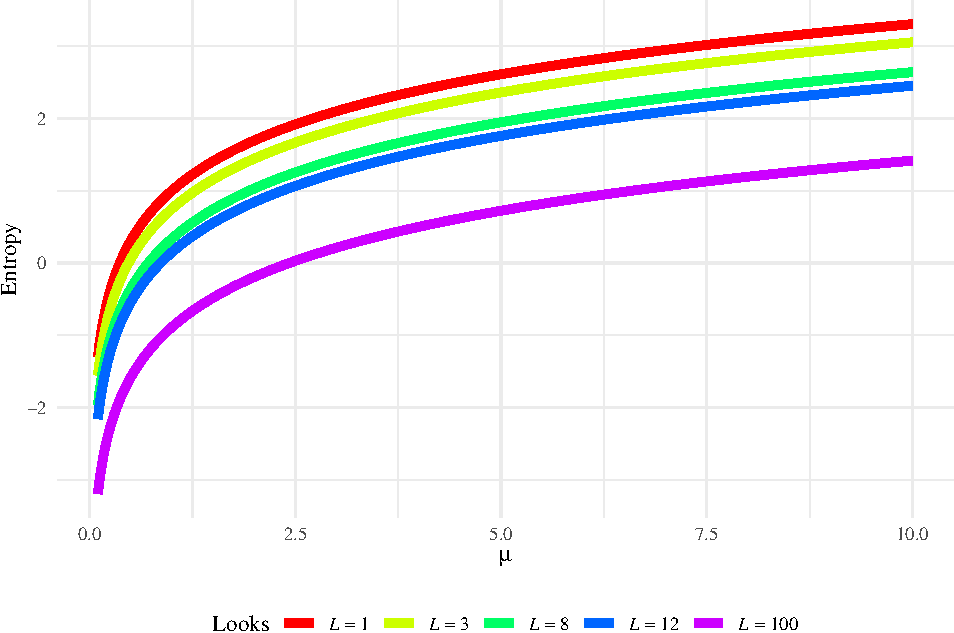
\includegraphics[width=1\linewidth]{R1-The-Entropy-as-a-Proxy-for-Fully-Developed-Speckle_files/figure-latex/PlotGammaSAR-1} 

}

\caption{The Shannon Entropy under the Gamma SAR model.}\label{fig:PlotGammaSAR}
\end{figure}

Fig.~\ref{fig:3d_GIO} illustrates the entropy of \(G_I^0\) distribution
as a function of three key parameters: \(\mu\), \(\alpha\), and \(L\).

\begin{figure}[hbt]

{\centering 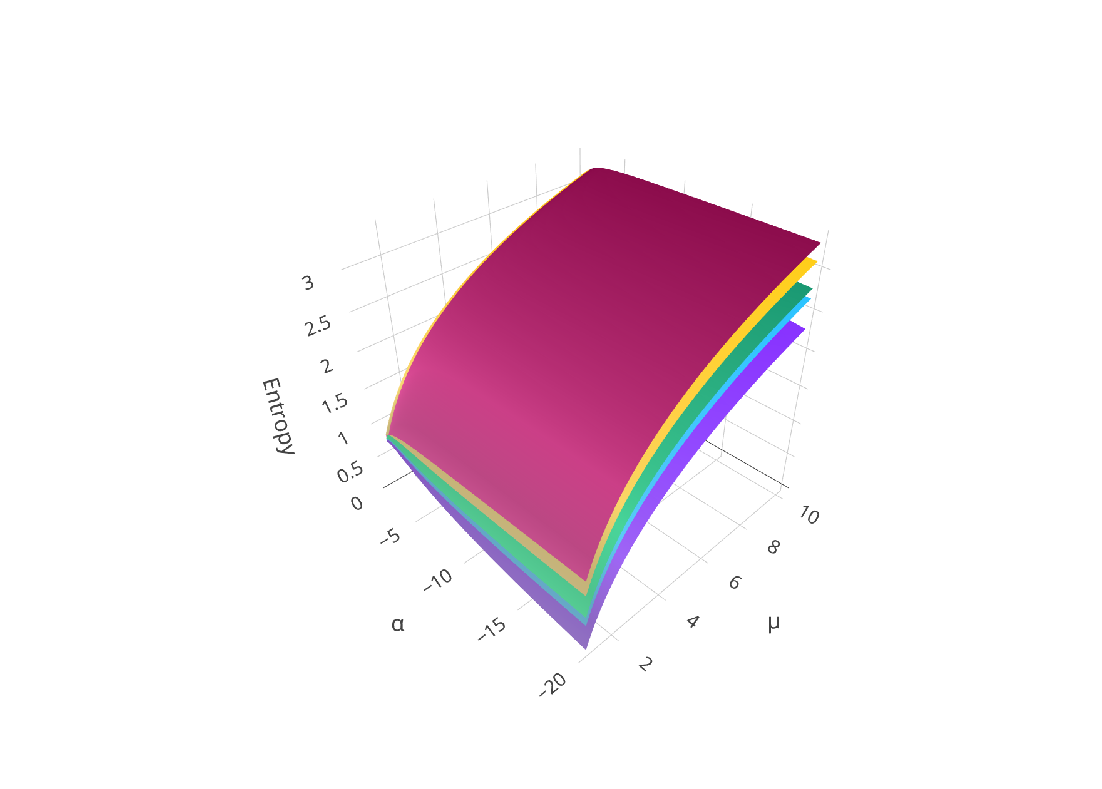
\includegraphics[width=0.7\linewidth]{../../../Figures/PDF/entropy_plot_3d} 

}

\caption{The Shannon Entropy under ${G}_I^0$ models.}\label{fig:3d_GIO}
\end{figure}

As we explore the 3D plot, we can observe how changes in \(\mu\),
\(\alpha\), and \(L\) collectively influence the entropy of the
\(G_I^0\) distribution. We can identify regions where entropy is high or
low, providing insights into the predictability and structure of the
distribution in various regions of the parameter space.

\hypertarget{estimation-of-the-shannon-entropy}{%
\subsection{Estimation of the Shannon
Entropy}\label{estimation-of-the-shannon-entropy}}

One of the earliest non-parametric estimators relying on spacings was
introduced by~\cite{vasicek1976test}. Assuming that
\(\bm{Z}=(Z_1, Z_2,\ldots,Z_n)\) is a random sample from the
distribution \(F(z)\), the estimator is defined as: \begin{equation*}
\label{E:Vas}
    \widehat{H}_{\text{V}}(\bm{Z})=\frac{1}{n}\sum_{i=1}^{n}\ln\left[\frac{n}{2m}\left(Z_{(i+m)}-Z_{(i-m)}\right)\right],
    \end{equation*} where \(m<n/2\) is a positive integer,
\(Z_{(i+m)}-Z_{(i-m)}\) is the \(m\)-spacing and
\(Z_{(1)}\leq Z_{(2)}\leq\ldots\leq Z_{(n)}\) are the order statistics
and \(Z_{(i)}= Z_{(1)}\) if \(i<1\), \(Z_{(i)}= Z_{(n)}\) if \(i>n\).

Several authors have explored adaptations to Vasicek's estimator. In
this work, we consider three entropy estimators known for their superior
performance:

\begin{itemize}
\item
  \cite{correa1995new}: \(\widehat{H}_{\text{C}}\).
\item
  \cite{Ebrahimi1994}: \(\widehat{H}_{\mathrm{E}}\).
\item
  \cite{IbrahimAlOmari2014}: \(\widehat{H}_{\mathrm{AO}}\).
\end{itemize}

These estimators, along with others, are described and studied
in~\cite{Cassetti2022}.

\hypertarget{enhanced-bootstrap-technique}{%
\subsection{Enhanced Bootstrap
Technique}\label{enhanced-bootstrap-technique}}

We employ the bootstrap technique to refine the precision of existing
non-parametric entropy estimators. This approach involves generating new
datasets through resampling with repetition from an existing one.

Let's assume that non-parametric entropy estimators
\(\widehat{H}=\widehat{\theta}(\bm{Z})\) are inherently biased, that is:
\begin{equation}
\label{Eq:bias1}
\operatorname{Bias}\big(\widehat{\theta}(\bm{Z})\big) = E\big[\widehat{\theta}(\bm{Z})\big] - \theta.
\end{equation} Our objective is to devise unbiased estimators with
reduced variance. To achieve this, we introduce an ``ideal estimator''
\(\check{\theta}(\bm{Z})\) using the bias information: \begin{equation}
\label{Eq:bias2}
\widecheck{\theta}(\bm{Z}) = \widehat{\theta}(\bm{Z}) - \operatorname{Bias}\big(\widehat{\theta}(\bm{Z})\big).
\end{equation} However, \(\check{\theta}(\bm{Z})\) is not an estimator,
because it depends on the true parameter \(\theta\), prompting the
formulation of a new estimator \(\widetilde{H}\). From \eqref{Eq:bias1}
and \eqref{Eq:bias2} we have: \begin{align*}
\widetilde{H} &= 2\widehat{\theta}(\bm{Z}) - \frac{1}{B}\sum_{b=1}^B \widehat{\theta}_b(\bm{Z}^{(b)}),
\end{align*} where \(B\) is the number of replications in the bootstrap
technique. Applying this methodology, the original estimators by Correa,
Ebrahimi, and Al-Omari are now denoted as the proposed
bootstrap-enhanced versions: \(\widetilde{H}_{\text{C}}\),
\(\widetilde{H}_{\text{E}}\), and \(\widetilde{H}_{\text{AO}}\),
respectively.

\hypertarget{sec:test}{%
\section{Hypothesis testing based on non-parametric
entropy}\label{sec:test}}

General asymptotic results for functions of spacings are
detailed~\cite{Khashimov1990}, while~\cite{Bert1992} developed a
correction for the case of Shannon entropy. Following the work of these
authors, the next result applies:

\begin{lemma}
Suppose that $f(\cdot)$ is a bounded density bounded away from zero and satisfies a Lipschitz condition on its support.
Then, if $m,n\rightarrow \infty$ and $m=o(n^{1/2})$, holds that:
\begin{equation*}
\sqrt{n}\,\Big(\label{Eq:bias_t}
\widetilde{H}_{i}+\int_{-\infty}^\infty f(z)\ln f(z) \mathrm{d}z\Big)
\xrightarrow[]{\mathcal{D}}
\mathcal{N}(0,\operatorname{Var}(\ln f(Z))).
\end{equation*}
\end{lemma}

Consider, starting from the previous lemma, the test of the null
hypothesis \(\mathcal{H}_0: T_{\mathcal{D}}=D_0\) as opposed to one of
the other three: \begin{align*}
\mathcal{H}_1 &: T_{\mathcal{D}}\neq D_0,\\ 
\mathcal{H}_1 &: T_{\mathcal{D}}> D_0,\text{ or}\\
\mathcal{H}_1 &: T_{\mathcal{D}}< D_0. 
\end{align*} For this purpose, we can use the test statistics:
\begin{equation*}
Z_{m,n} = \frac{\sqrt{n}\big(\label{Eq:bias4}
\widetilde{H}-D_0\big)}{\sqrt{\operatorname{Var}\big(\ln f(Z)\big)}},
\end{equation*} so the null hypothesis should be rejected if (i)
\(Z_{n,m} > z_{\alpha/2}\) or \(Z_{n,m} < - z_{\alpha/2}\) for
\(\Phi_{\mathcal N}(z_{\alpha/2})=1-\alpha/2\) and \(\Phi_{\mathcal N}\)
being the standard normal cumulative distribution function, (ii)
\(Z_{n,m} > z_{\alpha/2}\) or (iii) \(Z_{n,m} < - z_{\alpha/2}\).

The power function for case (i) (two-sided test) at \(t\neq D_0\) is
given by \begin{multline*}
\pi_{m,n}(t)=1-\Phi_{m,n}\Big(z_{\alpha/2}-\frac{\sqrt{n}(Z_{m,n}-D_0)}{\sigma}\Big)\\+\Phi_{m,n}\Big(-z_{\alpha/2}-\frac{\sqrt{n}(Z_{m,n}-D_0)}{\sigma}\Big),
\end{multline*} for a sequence of cumulative distribution functions
\(\Phi_{m,n}(x)\) which tends uniformly to \(\Phi_{\mathcal N}(z)\).

\hypertarget{sec:results}{%
\section{Results}\label{sec:results}}

Simulations are conducted using \(G_I^0\) distribution, with \(200\)
simulated samples of size \(n\in\left\{9, 25, 49, 81, 121\right\}\),
with parameters \(\mu \in \left\{1, 10\right\}\), \(\alpha=-20\), and
\(L=8\). In the case of the bootstrap technique, each sample is
replicated \(100\) times with replacement. We choose to use the
following heuristic formula for spacing,
\(m=\left[\sqrt{n}+0.5\right]\).

In Fig. \ref{fig:Plot_bias_mse_gi0} we depict comparisons of bias and
mean squared error (MSE) between the original non-parametric entropy
estimators and their respective bootstrap-enhanced versions. The use of
the bootstrap technique exhibits more precision, reduced bias and MSE,
and improved convergence.

The results of simulation are exhibited in Table~\ref{tab:table2}. The
precision of estimators, as evidenced by bias and MSE comparisons,
benefits significantly from the bootstrap technique, particularly for
sample sizes below 81.

\begin{figure}

{\centering 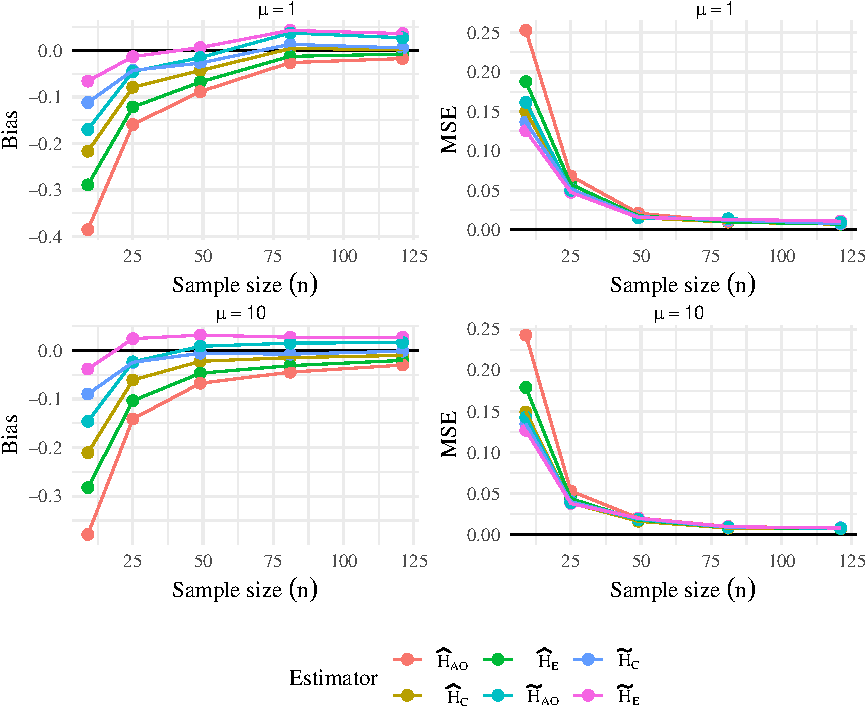
\includegraphics[width=1\linewidth]{R1-The-Entropy-as-a-Proxy-for-Fully-Developed-Speckle_files/figure-latex/Plot_bias_mse_gi0-1} 

}

\caption{Bias and MSE of entropy estimators for  $G_I^0$, $L=8$, $\alpha=-20$.}\label{fig:Plot_bias_mse_gi0}
\end{figure}

\begin{table}

\caption{\label{tab:table2}Bias and MSE of bootstrap estimators for $G_I^0$, $L=8$, $\alpha=-20$.}
\centering
\begin{tabular}[t]{cccccccc}
\toprule
\multicolumn{1}{c}{ } & \multicolumn{1}{c}{ } & \multicolumn{3}{c}{Bias} & \multicolumn{3}{c}{MSE} \\
\cmidrule(l{3pt}r{3pt}){3-5} \cmidrule(l{3pt}r{3pt}){6-8}
$\bm{\mu}$ & $\bm{n}$ & $\widetilde{H}_{\text{C}}$ & $\widetilde{H}_{\text{E}}$ & $\widetilde{H}_{\text{AO}}$ & $\widetilde{H}_{\text{C}}$ & $\widetilde{H}_{\text{E}}$ & $\widetilde{H}_{\text{AO}}$\\
\midrule
 & 9 & -0.1117 & -0.0657 & -0.1698 & 0.1367 & 0.1255 & 0.1616\\

 & 25 & -0.0428 & -0.0131 & -0.0451 & 0.0515 & 0.0474 & 0.0499\\

 & 49 & -0.0267 & 0.0065 & -0.0152 & 0.0165 & 0.0154 & 0.0151\\

 & 81 & 0.0134 & 0.0434 & 0.0377 & 0.0121 & 0.0133 & 0.0138\\

\multirow{-5}{*}{\centering\arraybackslash 1} & 121 & 0.0055 & 0.0364 & 0.0275 & 0.0078 & 0.0108 & 0.0092\\
\cmidrule{1-8}
 & 9 & -0.0900 & -0.0386 & -0.1463 & 0.1345 & 0.1268 & 0.1427\\

 & 25 & -0.0247 & 0.0239 & -0.0239 & 0.0399 & 0.0378 & 0.0388\\

 & 49 & -0.0060 & 0.0312 & 0.0082 & 0.0194 & 0.0198 & 0.0183\\

 & 81 & -0.0080 & 0.0270 & 0.0147 & 0.0088 & 0.0095 & 0.0088\\

\multirow{-5}{*}{\centering\arraybackslash 10} & 121 & -0.0019 & 0.0267 & 0.0160 & 0.0080 & 0.0078 & 0.0075\\
\bottomrule
\end{tabular}
\end{table}

\begin{table}

\caption{\label{tab:table_hipotesis}Hypothesis Testing for $G_I^0$, $\mu = 5 $, $L=2$, $\alpha=-1000$ , $H_{\Gamma_{\text{SAR}}}=2.493$.}
\centering
\begin{tabular}[t]{ccccc}
\toprule
$n$ & Estimator & Mean Entropy & $Z$ Statistic & $p$ Value\\
\midrule
 & $\widetilde{H}_{C}$ & 2.4689 & -0.6699 & 0.5029\\

 & $\widetilde{H}_{E}$ & 2.5080 & 0.3764 & 0.7066\\

\multirow{-3}{*}{\centering\arraybackslash 9} & $\widetilde{H}_{AO}$ & 2.4119 & -2.2774 & 0.0228\\
\cmidrule{1-5}
 & $\widetilde{H}_{C}$ & 2.4713 & -1.1379 & 0.2552\\

 & $\widetilde{H}_{E}$ & 2.5000 & 0.3392 & 0.7344\\

\multirow{-3}{*}{\centering\arraybackslash 25} & $\widetilde{H}_{AO}$ & 2.4551 & -1.9487 & 0.0513\\
\cmidrule{1-5}
 & $\widetilde{H}_{C}$ & 2.4515 & -3.1650 & 0.0015\\

 & $\widetilde{H}_{E}$ & 2.4882 & -0.4299 & 0.6673\\

\multirow{-3}{*}{\centering\arraybackslash 49} & $\widetilde{H}_{AO}$ & 2.4726 & -1.5996 & 0.1097\\
\cmidrule{1-5}
 & $\widetilde{H}_{C}$ & 2.4937 & 0.0159 & 0.9873\\

 & $\widetilde{H}_{E}$ & 2.5262 & 2.8534 & 0.0043\\

\multirow{-3}{*}{\centering\arraybackslash 81} & $\widetilde{H}_{AO}$ & 2.4974 & 0.3594 & 0.7193\\
\cmidrule{1-5}
 & $\widetilde{H}_{C}$ & 2.4922 & -0.1442 & 0.8853\\

 & $\widetilde{H}_{E}$ & 2.5169 & 2.5684 & 0.0102\\

\multirow{-3}{*}{\centering\arraybackslash 121} & $\widetilde{H}_{AO}$ & 2.5052 & 1.3283 & 0.1841\\
\bottomrule
\end{tabular}
\end{table}

A hypothesis testing was conducted using non-parametric entropy
estimators as test statistics. The results in
Table~\ref{tab:table_hipotesis} show that data from the \(G_I^0\)
distribution exhibit fully developed speckle behavior, specifically in
the limit case with parameters \(\mu=5\), \(L=2\), and
\(\alpha= -1000\). The true entropy of \(\Gamma_{\text{SAR}}\) was set
at \(H_{\Gamma_{\text{SAR}}} = 2.493\).\\
It is observed that, for different sample sizes, entropy values converge
towards the true value of the Gamma SAR distribution. Hypothesis test
results were conducted with a \SI{95}{\percent} confidence level. The
\(Z\) statistic measures the discrepancy between the estimated entropy
and the true entropy. The \(p\)-values associated with the \(Z\)
statistic are predominantly greater than \(0.05\), for sample sizes
above \(25\), suggesting that the data are consistent with the null
hypothesis.

\hypertarget{sec:conclusion}{%
\section{Conclusion}\label{sec:conclusion}}

In this study, three estimators renowned for their robust performance
across diverse distributions were chosen for evaluation. We examine the
impact of applying bootstrap techniques on their precision by comparing
each estimator's performance with its bootstrap-enhanced counterpart,
utilizing metrics such as bias and MSE. The effectiveness of
bootstrap-enhanced non-parametric entropy estimators was observed,
demonstrating efficacy in most instances. Nonetheless, it is essential
to recognize that the applicability of this technique may not be
universal across all estimation methods.

It is worth noting that this analysis represents an initial exploration
of SAR Intensity data, and future work will include a more in-depth
analysis of effect size and statistical power. Additionally, exploring
the impact of the \(\alpha\) parameter on estimates and conducting more
extensive analyses to assess the generalization of results to different
parameter configurations is suggested.

\renewcommand\refname{References}
\bibliography{../../Common/references.bib}
\end{document}

